\documentclass{article}

\usepackage[utf8]{inputenc}
\usepackage{authblk} % authors

\usepackage{lineno} % used along with \linenumbers after begin document. 
\usepackage{setspace} % line spacing
  \setstretch{1.4}
\usepackage{enumitem}
\usepackage{microtype} % Creates better spaced text
\usepackage{siunitx} % SI units 

\usepackage{xcolor} % Setting colours and their usage
  \definecolor{natureblue}{RGB}{5,110,210}

\usepackage[colorlinks]{hyperref} % Colour for hyperlinks, (URLs, citations, cross reference)
  \AtBeginDocument{%this allows colours to change from the defined article template.
  \hypersetup{
  linkcolor={natureblue},
  citecolor={natureblue},
  filecolor=blue!50!black,
  urlcolor=natureblue,
  }}

\usepackage{natbib}
  \setcitestyle{square,numbers,sort&compress}
  \setcitestyle{sort&compress}
\usepackage{hypernat} % hypernat also required to allow citations to compress. 
\usepackage{graphicx}
\graphicspath{ {images/} } % sets the path to image files (Figures)

\usepackage{booktabs} % required for tables
\usepackage{rotating,tabularx} % tabularx is the table style used, rotating can also be used
\newcolumntype{Z}{ >{\centering\arraybackslash}X } % defining table content layout per box
\usepackage{ltablex} % allow page break between lines in tabularx
\usepackage{caption} \captionsetup{font=normalsize} % to set the caption size as normal even when table is tiny.

\usepackage{pdflscape} % for rotated table
\usepackage{multirow} % for table

\begin{document}
\date{} %don't want date printed
%make title bold and 14 pt font (Latex default is non-bold, 16 pt)
\title{\Large \bf Viral genetic determinants of persistent human orthopneumovirus infection.
\footnote{This document's private source code is available to co-authors from the 
\href{https://github.com/DylanLawless/inspire_manscript}{GitHub repository}, from the 
\href{https://www.overleaf.com/project/61718a4e077acc3d20ee68f1}{Overleaf online editor document}, or as MS Word format on box. The completed document will be published on 
\href{https://www.biorxiv.org}{biorxiv} or \href{https://www.medrxiv.org}{medrxiv} before journal submission.
All code used in this project will be available on the 
\href{https://github.com/DylanLawless/inspire_manscript}{GitHub repository} and supplemented with "toy" data.}
}
%\thanks {Use thanks if u you need it}
%for single author (just remove % characters)

\author[1]{\rm Dylan Lawless, PHD}
\author[2]{\rm Christopher G. McKennan, PhD}
\author[]{\rm Suman Das, PhD}
\author[]{\rm Larry J Anderson}
\author[]{\rm  Tebeb Gebretsadik}
\author[]{\rm Meghan Shilts}
\author[]{\rm Christian Rosas-Salazar}
\author[3]{\rm James D. Chappell, MD}
\author[1]{\rm Jacques Fellay, MD, PhD }
\author[3,4]{\rm Tina V. Hartert, MD, MPH}

\affil[1]{Global Health Institute, School of Life Sciences, École Polytechnique Fédérale de Lausanne, Lausanne, Switzerland}

\affil[2]{Department of Statistics, University of Pittsburgh, Pittsburgh, Pennsylvania, United States of America}

\affil[3]{Department of Pediatrics, Vanderbilt University Medical Center, Nashville, Tennessee, United States of America}
\affil[4]{Department of Medicine, Vanderbilt University Medical Center, Nashville, Tennessee, United States of America}

%\affil[ ]{\textit {\{email1,email2,email3,email4\}@xyz.edu}}
\maketitle

% CID - clinical spin, Jim describes other good examples in this journal. Up to 5 keywords  Word limit: 3000 words (excluding the abstract and references). Key points should be summarized on the title page in 40-words or less. Abstract: Up to 250 words. Tables/Figures: As required / No max? References: 40 or less. References should be numbered consecutively, in brackets on the text line (e.g., [3, 7–9, 57]). For references with more than 6 authors, the first 3 authors should be listed, followed by et al. 
% % <!-- ## Backups -->
% <!-- * JID -  would probably do well here. -->
% <!-- * PLOS pathogens - Good quality but could be a little slower. -->
% <!-- * Journal of virology. -->

\linenumbers
\subsection*{Abbreviations}
ALT (alternative);
CI (confidence interval);
GWAS (genome-wide association study);
G (glycoprotein);
H (hemagglutinin);
HN (hemagglutinin-neuraminidase);
IFN (interferon);
IQR (interquartile range);
INSPIRE (The INfant Susceptibility to Pulmonary Infections and Asthma Following RSV Exposure in Infancy Birth Cohort);
LD (linkage disequilibrium);
MSA (multiple sequence alignment);
OR (odds ratio);
PCR (polymerase chain reaction);
PCA (Principal component analysis);
REF  (reference);
RT (reverse transcription);
SVD (singular value decomposition);
VE (variance explained);
MSA (multiple sequence alignment);
RSV (respiratory syncytial virus).

\section{Abstract}
1. RSV world health.
2. Viral genome sequencing and host contributing features.
3. Control for all know interactions.
4. Here we identify RSV variants that are associated with persistent infection.
5. Conclusion

\section{Introduction}
Respiratory syncytial virus (RSV), a human orthopneumovirus, is the single most important respiratory virus resulting in the most significant respiratory morbidity and mortality in infants 
\cite{hall_burden_2009}.
By the age of 2 years, nearly all children are infected with RSV at least once 
\cite{glezen_risk_1986}.
RSV infects primarily the upper and lower respiratory tract epithelium, although has been recovered from non-airway sources 
\cite{bokun_respiratory_2019,
cubie_detection_1997,
nadal_isolation_1990,
odonnell_respiratory_1998,
rezaee_respiratory_2011,
rohwedder_detection_1998}.
Prolonged shedding of RSV, especially in young infants and following first infection, has been demonstrated, with longer average duration of viral shedding using polymerase chain reaction (PCR) to detect RSV 
\cite{munywoki_influence_2015}.
While younger age and first infection are associated with persistence of infection, what isn't understood is whether there are viral factors contributing to prolonged shedding or persistence of RSV in young infants. 
This is important, as persistent infection, or prolonged shedding may contribute to enhanced transmission and developmental changes to the early life  airway epithelium. 
Further, the reservoir of RSV infection is not understood, 
and it is possible that some RSV strains and/or hosts could serve as a dormant reservoir for infection that is activated by seasonal or other influences 
\cite{hobson_persistent_2008}.
Further, host genetic and viral genetic interactions have never been studied for RSV.
With increasing adoption of human genomics in parallel with pathogen sequencing, novel methods for genome-to-genome analysis provide opportunities to identify selective pressure between host and pathogen \cite{naret2018correcting}.
We have previously investigated host genetics as a source of acceptability to infection (summarise result) (cite).
Several environmental factors have a significant impact on the risk of infection. 
Population genetics also contributes important features that must be accounted for during genetics association analysis. 
These features not only depend on the host genetics as seen within a typical genome-wide association study (GWAS), but also depend on the viral genetics.
RSV strains A and B impart the largest separation within the viral population phylogeny.
In this study we perform genomic analysis of RSV to identify variants that are significantly associated with persistent infection in otherwise healthy children.

\section{Methods}
\subsection{Study population}
The protocol and informed consent documents were approved by the Institutional Review Board at Vanderbilt University Medical Center. 
One parent of each participant in the cohort study provided written informed consent for participation in this study. 
The informed consent document explained study procedures, use of data and biospecimens for future studies, including genetic studies.

The study population is a longitudinal birth cohort - The INfant Susceptibility to Pulmonary Infections and Asthma Following RSV Exposure in Infancy Birth Cohort (INSPIRE) - specifically designed to capture the first RSV infection during infancy in a term healthy birth cohort. 
Additional details of this birth cohort has been previously published 
\cite{larkin_objectives_2015}.
Briefly, the cohort includes 1952 term ($\ge$ 37 weeks gestation), non-low birth weight ($\ge$ 2250 g, 5 lbs), otherwise healthy infants from a population-representative sample from pediatric practices located in a rural, suburban, and rural region of the southeastern US during 2012-2014. 
Infants were born June through December so that they would, by design, be 6 months of age or less entering their first RSV season. 
Infant (i.e., the first year of life) RSV infection was ascertained through passive and active biweekly surveillance during each infants' first RSV season and RSV serology
(Table \ref{tab:1}).

\subsection{Biweekly surveillance of RSV infection}
To capture all RSV infections of children enrolled in INSPIRE throughout infancy (i.e., the first year of life), we conducted passive and active surveillance during their first RSV season by 1) performing bi-weekly phone, email, and/or in person follow-up, 2) frequently educating and reminding parents to call us at the onset of any acute respiratory symptoms, and 3) approaching all infants who were seen at one of the participating pediatric practices for an unscheduled visit. 
If an infant met pre-specified criteria for an acute respiratory infection, we then conducted an in-person respiratory illness visit at which time we administered a parental questionnaire, performed a physical exam, collected a nasal wash, and (in infants seen during an unscheduled visit) completed a structured medical chart review.
Nasal sample collections were assessed by reverse transcription-quantitative PCR for RSV [Jim to provide reference].
At one year of age infants underwent blood draw for RSV serology to determine infection status during infancy. 
[Plots with CT-value from Tina, either as supplemental or first mention later so not to pollute the order].
Infants with positive PCR separated by 15 or more days were annotated during analysis as "persistent or repeat infection"
(Figure \ref{fig:1}).

\subsection{Descriptive analyses}
Descriptive analyses of the cohort were conducted using R 4.0.5 (available at: 
\url{http://www.r-project.org}). 
Pearson or Wilcoxon tests were used for comparing infants with and without persistent RSV infection.
The main descriptive features are provided in 
Table \ref{tab:1}.
[Consider plotting these also in the Hmisc Harrell style as seen in his book, RegerssionModellingStrategies2015].

\subsection{RSV whole-genome sequencing}
RSV whole-genome sequencing of this study population has been previously described 
\cite{schobel_respiratory_2016}.
Briefly, RNA was extracted at J. Craig Venter Institute (JCVI) (\url{https://www.jcvi.org}) in Rockville, MD from nasal wash samples which were RSV PCR positive and collected during a respiratory illness visit triggered through biweekly surveillance of symptoms. 
Four forward reverse transcription (RT) primers were designed and four sets of PCR primers were manually picked from primers designed across a consensus of complete RSV genome sequences using JCVI’s automated primer design tool,
\cite{li_automated_2012}.
cDNA was generated from \SI{4}{\micro\liter}  undiluted RNA, using the pooled forward primers and SuperScript III Reverse Transcriptase (Thermo Fisher Scientific, Waltham, MA, USA). 
100 ng of pooled DNA amplicons were sheared to create 400-bp libraries, which were pooled in equal volumes and cleaned. 
For samples requiring extra coverage, in addition to Ion Torrent sequencing, Illumina libraries were prepared using the Nextera DNA Sample Preparation Kit (Illumina, Inc., San Diego, CA, USA). 
Sequence reads were sorted by barcode, trimmed, and de novo assembled using CLC Bio's \textit{clc\_novo\_assemble} program, and the resulting contigs were searched against custom, full-length RSV nucleotide databases to find the closest reference sequence. 
All sequence reads were then mapped to the selected reference RSV sequence using CLC Bio's \textit{clc\_ref\_assemble\_long} program 
\cite{bioWhite2016}.
% <!-- \cite{bioWhite2010} redundant v3.0 removed to reduce citations -->
Curated assemblies were validated and annotated with the viral annotation software called Viral Genome ORF Reader, VIGOR 3.0 (\url{https://sourceforge.net/projects/jcvi-vigor/files/}), before submission to GenBank as part of the Bioproject accession PRJNA225816 (\url{https://www.ncbi.nlm.nih.gov/bioproject/225816})
% <!--(30-Oct-2013 73 samples)-->
\cite{wang_vigor_2012} 
and PRJNA267583 (\url{https://www.ncbi.nlm.nih.gov/bioproject/267583}).
% <!--(17-Nov-2014 264 samples)-->

\subsection{Viral Sequence alignment}
% <!---_Sequence data format:_--->
% <!---sqn--->
The NCBI-tools Tbl2asn (\url{https://www.ncbi.nlm.nih.gov/genbank/tbl2asn2/})
was used in the creation of sequence records for submission to GenBank (\url{https://www.ncbi.nlm.nih.gov/genbank/}).
A total of 350 viral sequences in \textit{.sqn} file format were used for downstream analysis.

% <!---_Fasta format:_--->
% <!---fa--->
We computed a phylogenetic tree for each gene, as follows.
NCBI-tools asn2fsa (\url{https://www.huge-man-linux.net/man1/asn2fsa.html}) was used to to convert to fasta format.
% <!--- /work/gr-fe/lawless/inspire/rsv_viral_seq/ 1.export_nucleotide.sh --->
% <!--- 2.simplify_header.sh --->
% <!---_Data curation:_--->
% <!---seg_master/ Mar 3rd--->
Each sample consisted of 11 sequence segments
(NS1, NS2, N, P, M, M2-1, M2-2, SH, G, F, and L) as shown in 
Figure \ref{fig:1}.
These were separated and repooled to create 11 single fasta files for each gene containing all 350 samples. 
% <!---split_seg.sh --->
% <!---With awk, I split each fasta to a new file and labeled with the real name. i.e. segment 1 for all samples is in the file seg\_1, etc. dir: ./seg--->
Sequences were checked that they also be at least 90% as long as the maximum length 
for the corresponding gene in order to minimize the loss of aligned positions when computing the phylogenetic tree. 
% <!---_Multiple seuqnce alignment:_--->
% <!---aln/ Feb 18th--->
Each of the eleven resulting sets was aligned with MAFFT v7 (\url{https://mafft.cbrc.jp/alignment/software/})
\cite{katoh2013mafft},
using default  parameters.
The sequence of the orthologous gene from the bovine orthopneumovirus 
(\href{https://www.ncbi.nlm.nih.gov/nuccore/NC_001989}{GenBank:NC\_001989}) 
was added to each set as an outgroup. 
% <!---
%pep (outgroup seq)
%msa (all aligned per gene)
%pep (fixed version of msa)
%--->
% <!---  clw/ Jan 28th (Muscle alignment) Not used by Thomas --->
% <!--- nex/ Jan 30thI don't think this was used.  One nexus file per gene. It stores information about taxa, morphological and molecular characters, distances, genetic codes, assumptions, sets, trees, etc. --->

% <!---_Phylogenetic tree:_--->
% <!---nw/ Mar 10th--->
IQ-Tree 
(\url{https://www.iqtree.org})
\cite{nguyen2015iq}
was used with per-gene multiple sequence alignment (MSA) files for estimating maximum-likelihood phylogenies.
% <!---Analysis results written to:
%IQ-TREE report:                M2-2_new_wOG.msa.iqtree¬
%Maximum-likelihood tree:       M2-2_new_wOG.msa.treefile¬
%Likelihood distances:          M2-2_new_wOG.msa.mldist¬
%Screen log file:               M2-2_new_wOG.msa.log¬
%msa
%msa.bionj
%msa.ckp.gz
%msa.iqtree
%msa.log
%msa.mldist
%msa.model.gz
%msa.treefile
%msa.uniqueseq.phy 
%--->
% <!---_Alignment Quality:_--->
Examining the sequences with an alignment viewer showed that X sequences 
had frame shift variants but which did not affect the regions included in our testing criteria.
% <!--Discuss whether anything extra is needed for these sequences; e.g. alignments recomputed until no frame shifts were observed.-->
% <!---
%\subsection{Analysis order of code}
%1. update_G_phylogeny_nucleic_acid_msa_logist_data_prep_covariates.R
%2. update_G_phylogeny_nucleic_acid_msa_logist_covariates.R source(1)
%3. update_G_pca.R source(1+2)
%4. update_G_LD source(1)
%5. asthma_and_candidate_variant_lm (no sig results, remove)
%6. public_data
%--->

% <!-- ## Data merged and cleaned -->
% <!--Label repeat infections -->
Viral sequence data and clinical information was merged and cleaned with R.
Clinical IDs matching more than one viral sequence IDs were used to label "repeat or persistent" infections. 
Genetic variation was quantified in these samples and for subsequent analysis, only the first viral sequence was included for association testing. 
Strain A and B typing had been completed previously and labels were included to annotate each sample accordingly.

The cohort-specific variant frequency per position was calculated;
residues were counted and ranked by frequency,
with the most frequent residue defined as reference (REF) or alternative (ALT).
Positions with at least one ALT were checked for potential misalignment or other sources of error. 
Variants positions were selected for association analysis, while non-variant position were ignored.

A number of host features have been previously shown to influence infection susceptibility and were therefore included as covariates in our analysis (cite Rosas-Salazar).
Six samples were excluded due to insufficient covariate data, resulting in 344 test samples. 
Of these, 36 were from the same patients ("persistent or repeat" infection) of which half (18) were included for association testing; 326 samples total.
% <!--Correlations viewed with: corrplot, ggcorrplot, caret.-->


\subsection{Population structure}
The genetic distances to nearest neighbors were computed based on phylogenetic 
trees generated with MAFFT.
[Other methods also used but not pertinent; include some info from the code].
Principal component analysis (PCA) and singular value decomposition (SVD) were used in dimensionality reduction for exploratory data analysis of viral phylogeny.
R package \textit{factoextra} was used for PCA, and to visualise eigenvalues and variance. 
R package \textit{caret} was used to analyse genetic correlations.

\subsection{Association testing}
Viral amino acids (genotype collapsed into REF/ALT) were tested for association with infection types \textit{single} and \textit{persistent}, 
including key covariates that are significantly associated with infection.
Analysis was performed using logistic regression with the
R stats (3.6.2) \textit{glm} function as a generalized linear model.
The model consisted of the binary response (persistent infection Yes/No), and predictors; viral genotype (REF/ALT amino acid), viral PCs 1-5, host sex, and it also accounted for host features that have been previously demonstrated as significantly associated with infection; 
self-reported race/ethnicity, child-care attendance, living with siblings (cite Rosas-Salazar).

% $ glm(\text{Infection status} \text{\textasciitilde} \text{genotype} + \text{PCs} + \text{birth month} + \text{sex} + \text{race} + \text{child-care} + \text{siblings}, \text{family} = \text{'binomial'}) $

% <!---
% Logistic regression models are often used to analyse binary data (e.g. disease status), and can be described in the generalised linear model framework. 
% Suppose that $y_i$ is the realisation of a random variable 
% $Y_i$ for the 
% $i$-th individual, 
% where $Y_i = 1$ if the individual has the disease and 0 otherwise. 
% $Y_i$ is assumed to be Bernoulli distributed,

% $$ Y_i ∼ \text{Bernoulli}(\pi_i), $$

% with probability $\pi_i$. 
% In logistic regression, the logit link function is used to relate the underlying probability $\pi_i$ to a linear function of the predictors,

% $$ 
% logit(\pi_i) = log (\frac{\pi_i}{1-\pi_i}) = x'_i \beta
% $$

% * where $x_i$ is the vector of covariates and 
% * $\beta$ is a vector of regression coefficients. 

% Maximum likelihood estimation is used to estimate the parameters in the model.
% Logistic regression in case-cohort studies applied directly to the cases and the subcohort noncases gives asymptotic inference of odds ratios.

% Logistic regression models were fitted using the glm package in R. 
% In the simulations, genotype and baseline age were included as covariates in the model. 
% That is,

% $$ 
% x'i\beta{} = \beta{}_A A_i + \beta{}_G G_i 
% $$

% where 
% * Ai is age measured in years for the i-th individual; 
% * $G_i$ is genotype for the i-th individual coded as 0, 1 or 2 according to the number of risk alleles; 
% * $\beta_A$ is the log(odds ratio) for a one year increase in age; 
% * and $\beta_G$ is the log(odds ratio) for a one allele increase in the risk allele. 

% In the applied example, the covariates included in the logistic regression models were the genotype of the genetic variant (coded as 0, 1 or 2 depending on the % number of risk alleles per individual), 
% * age (in years), 
% * sex, 
% * EPIC-CVD centre (as a categorical variable), 
% * and the first ten prinicipal components of ancestry.
% Conditional analysis.
% --->
The environmental host covariates did not contribute any significant effect in our model for the candidate-causal association.
Two viral PCs were included in our model for accuracy, however the clinical 
strain labels (A/B) also reflect the same cohort population structure.
[Check the \% VE from PC screen plot stats to 1 decimal place and list it here.]
Bonferroni correction for multiple testing was applied based on the number of independent variants tested.
R package \textit{stats} was used for a range of analysis including glm for logistic regressions. 
R package \textit{MASS} was used to analyse logistic regression model data.

% <!-- 
%\subsection{Strain definition and sub-analysis}
%Put sub-strain analysis into supplemental.
%Do we want to include anything else being done with this cohort?;
%RT-PCR, 
%serology, and genomic. 
%Strain sub-analysis.
%-->
Second infections occurred only in those with strain B. 
To test if the significantly associated variants were due to population structure, 
a subset of only strain B was performed. 
% Due to the smaller sample size the result no longer passed the significant threshold. 
% However, the same direct of effect indicated that the association was not a false positive. 
% OR and CI. 
% <!--
%\subsection{Variance over time in public data}
%-->

\subsection{Biological interpretation}
Some but not all of these methods will be included for our results section. 
Adjust based on discussion with co-authors.
Infant RSV infection results in decreased barrier function of the airway epithelium [cite].
Association between INF-gama and RSV amino acid position (w= wild vs A=alternatives) was adjusted for the same covariates as the main analysis. Wilcox test comparing interferon (IFN)-$\gamma$, and INF-$\alpha$, between RSV amino acid positions (W= wild type vs A=alternatives [3 combined]).
Protein structures were analysed with data sourced from 
RCSB PDB \url{https://www.rcsb.org}; Define the choice of PDB used. 
Protein function and doamins were assessed using 
UniProt	\url{https://www.uniprot.org}.
Interactions, PTM, motifs,and epitopes were assessed from literature. 
* Domain blast. 
* Multiple organism alignment - not complete.
Protein features were assessed using feature annotation data in bed file format from 
\url{https://www.ncbi.nlm.nih.gov}.
\paragraph{Figure and sup table of IFN response}

\section{Results}
\subsection{Cohort characteristics}
The INSPIRE cohort consisted of 1,949 enrolled infants 
(Figure \ref{fig:1}.).
Of these, 1,220 (~63\%) had $\ge$ 1 in-person respiratory illness visit(s). 
In total, there were 2,093 in-person respiratory illness visits completed and the median (interquartile range [IQR]) number of in-person respiratory illness visits per infant was 1 (1-2). 
% The characteristics of these infants compared with the other RSV infected infants and the entire cohort is shown in Table 1.
From the cohort, 344 RSV viral samples from 326 individuals were sequenced (methods).
There were 20 infants with RSV positive PCR $\ge$ 15 days apart who we suspected as having either persistent or repeat infection (based on genetic analysis).
% <!-- Also those who were sick enough to have a resp illness visit. --> 
Table \ref{tab:1} lists the cohort characteristics of infants with persistent RSV infection compared with other RSV infection and the entire cohort. 
Infection is defined as RSV sequence positive, with $\ge$ 15 days between testing. Pearson1, Wilcoxon2.
% <!-- There are other variables that we can include, although this seems sufficient. -->
[For Tebeb: We will need to recalculate this to represent just the first infection, as this small number infections include repeat infections which likely drives the median higher.]

The relatively small sample size of our cohort required analysis that targeted only genes which were \textit{a priori} likely to functionally contribute to the clinical phenotype. 
Therefore, our analysis focused on F and G glycoproteins (citations).
% <!-- [Include some points for our reasoning; -->
% <!-- Would we have false positives in other genes? -->
% <!-- We can interpret the results in F and G. -->
% <!-- These are the surface proteins that are most studied for vaccine development etc. -->
% <!-- Variation in other genes is lower; quntify this. --> 
% <!-- G and SH are variable more than others. -->
% <!-- M2 also has a fair amount of sequence variation. --> 
% <!-- F is more variable than others but maybe not the most so. --> 
% <!-- * Surface, entry, targets of immune response. --> 
% <!-- * F - Primary candidate for vaccine. --> 
% <!-- * Biological plausability is higher than others. --> 
% <!-- * G surface "glycoprotein", F - careful with terms. -->
% <!-- Larry / Suman can help. -->
% <!-- Their clinical relevance.] -->

\subsection{Population structure}
The phylogenetic tree based on G protein is shown in 
Figure \ref{fig:2} A.
One obvious feature causing a separation in genetic diversity is seen due to the G protein partial gene duplication, 
which has emerged in recent years within RSV-A strains 
\cite{eshaghi2012genetic}.
RSV-B strains with an analogous duplication have existed for two decades, 
although the mechanisms leading to emergence and clinical implications have not been entirely defined.

We observed persistent infections by viruses from different phylogenetic clades, rather than one specific clade 
Figure \ref{fig:2} B.
A genotype correlation matrix produced with the R package \textit{caret} and PCA and eignenvalues from package \textit{factoextra} were used for reducing the dimensionality of sequence data.
Figure \ref{fig:2} scree plot.
Dimension one accounted for 95.19\% cumulative variance explained in our cohort.
All other dimensions account for very little variance, which is evenly distributed; no particular F or G protein protein coding sequence separates the cohort.
          % <!-- eigenvalue variance.percent cumulative.variance.percent -->
% <!-- Dim.1   1.608637e+02     9.518559e+01                    95.18559 -->
For his reason, in our main analysis, viral population structure is accounted for by the first five PCs. 
To test for type I errors due to the population structure between strain A and B, 
a subset analysis of individual strains was performed to confirm the validity of the combined analysis.
% <!-- The main analysis was also repeated using viral strain labels A and B (separately derived from the clinical laboratory testing) instead of PCs which did not alter the analysis results, indicating no errors in sample handling. --> 

Note for presentation slides: there is no general theoretical reason that the most informative linear function of the predictor variables should lie among the dominant principal components of the multivariate distribution of the predictor variables. However, if there were then we would like to know since it would produce a false positive in this case. Conversely, for example, in a principal component regression you would hope to find the assoc based on PCs.

\subsection{Genetic invariance of persistent infection}
The duration of RSV shedding duration in Kenyan infants has been reported previously
\cite{okiro2010duration}.
 % <!-- \url{https://bmcinfectdis.biomedcentral.com/articles/10.1186/1471-2334-10-15#Sec1} -->
% <!-- This is the follow up. Ask Tina about the first paper too. --> 
Based on these finding, infections separated by at least 15 days were expected to be "new" infections. 
% <!-- In addition to our within-cohort genetic analysis showing --> 
Figure \ref{fig:2} C
shows genetic invariance between for viral sequences within the same host for infections separated by at least 15 days. 
There is a significant difference between the genetic diversity for multiple viral samples from individuals compared to diversity between all other samples from the same viral clades; $\text{P-value} = 1.3e-8$.
We therefore, report these cases as persistent infection rather than second infections.
% <!-- Have a look at update figure but the first version might be fine. --> 
% <!-- Complete. Check for other ways, criteria, variation within host doesn’t work since we don't have read data, only variant call. -->

\subsection{Variants in G glycoprotein significantly associated with persistent infection}
The consensus sequence within the cohort was assigned based on the major allele.
Variants at the amino acid level were defined as either REF/ALT and assessed for their association with persistence.
The model consisted of
the binary response (persistent infection Yes/No),
and predictors; viral genotype (REF/ALT amino acid), viral PCs 1-5, host sex, and it also accounted for host features that have been previously demonstrated as significantly associated with infection;
self-reported race/ethnicity, child-care attendance, living with siblings (cite).
Analysis was performed using R stats (3.6.2) \textit{glm} function. 
% <!-- glm ( infection ~ genotype + PCs + sex + other). -->
A significant genetic association was identified for persistent infection after Bonferroni correction multiple testing (threshold $<.05/23=.002$), 
as shown in 
Figure \ref{fig:3} A. 
Since many variants within RSV coding genes have non-random association due to strong linkage disequilibrium (LD), 
we reduced the multiple testing burden by retaining proxy variants and removing those with
$r^2 \ge .8$.
After identifying a significant association with persistent infection,
we quantified the correlation of variants in LD with the lead proxy.
% <!-- Conditional analysis was used to identify any independant signal. --> 
% <!-- Pruning, go through methods with Chris multiple test correction with threshold set at number of proxy SNVs rather than gene-wide SNV number. -->
Clumping was performed with ranking based on minor allele frequency (MAF) and with a cut-off threshold of $r^2 \ge .8$.
The association model was repeated for all variants to produce a Manhattan plot with $r^2$ by color and P-value statistics as shown in 
Figure \ref{fig:3} B.
This shows both G protein 
% <!-- "V126" --> 
p.E123K/D and 
% <!-- "V221" --> 
p.P217T/S/L as candidate causal variants associated with persistent infection, and no other variants in correlation with this association. 

To determine whether this association was simply due to population stratification between strains A and B, a subset analysis was performed using independently assessed clinical laboratory strain labels for A and B.
% <!-- Show how strains are defined in the genome sequence. --> 
% <!-- ## Shown not just false positive, accounting for population structure and strain, --> 
Due to the smaller sample size the result no longer passed the significant threshold. 
However, the same direct of effect indicated that the association was not a false positive. 
% State the OR in same direction with overlapping SE.

To assess the possibility of a false positive due to population structure within our cohort,
we assessed the magnitude of variance explained (VE) by the lead variant and found it as 
$-0.996\%$ VE for PC1 and $-1.66\%$ VE for PC2; 
a negligible effect that precludes spurious association by allele frequency between populations, as shown in 
Figure \ref{fig:3} C.

% <!-- We see that for 344 samples: --> 
% <!-- positions 280-300 = 80% variance in cohort. -->
% <!-- For a table, include average var expl for all variants. --> 
% <!-- Our variant of interest has extremely low %VE compared to the the top VE from PC1/PC2. -->
% <!-- This indicates that it is not a false positive due to a variant driving population structure. --> 
% <!-- | Var | PC | % VE | -->
% <!-- |-----|-----|-----| -->
% <!-- | 221 | PC1 | -0.996 | -->
% <!-- | 221 | PC2 | -1.66 | -->

% <!-- ## Variance explained over time, localised or general? --> 
% <!-- Phylogentic tree, eg 2016 paper. -->
% <!-- ## Public data -->
To investigate genetic variance over time
we assessed the public viral data repository of NCBI Human orthopneumovirus, taxid:11250 which contained data from 
27 unique countries worldwide, sample collection dates as far back as 1956, and 1084 glycoprotein protein sequences after curation.
We observed no enrichment for our variants of interest over time; 
a low frequency was observed in the available samples with no particular features compared to other low frequency variants. 
However, correlation between the two positions associated with persistent infection indicates that it does not arise as random mutation event.

% <!-- We already know it is not denovo in induals. -->
% <!-- Is our candidate persisting over time or is it arising repeatedly. -->
% <!-- We may be able to see this by looking at surrouding variation over time. -->
% <!-- The phylo tree shows the variant split over subgroups, only in B strain. --> 
% <!-- Spend some time listing the possibilities, facts we have, and facts that are missing. -->
% <!-- Discuss with Jim again. --> 
% <!-- Our variant over time did not reveal anything special. -->
% <!-- However, other parts of the gene are illuminating. --> 
% <!-- For example we can clearly see the introduction of G gene duplication, --> 
% <!-- and other parts of the gene that explain variation explained over time. --> 
% <!-- We can discuss if we want to mention the visibility of G gene duplication, --> 
% <!-- which is the most obvious feature. -->

% <!-- Don't think it could arise in a host over infection. --> 
% <!-- Chirs was saying because of LD it couldn't be the case. -->
% <!-- But not certain about the LD yet. --> 
% <!-- Need to look at the methods again for this. --> 

\subsection{Functional interpretation}
The main features of RSV surface glycoprotein are illustrated in Figure \ref{fig:5}.
There are no known features that directly overlap with the variant associated with persistent infection in our cohort. 
However, possible binding interactions with host receptors are discussed in (cite).
%Look at function of variants, 3d structure, etc.
(Reword) Attachment of the virion to the host cell membrane is thought to occur through interaction with heparan sulfate as shown in Figure \ref{fig:5}
(p.187-198), thereby initiating infection 
\cite{levine1987demonstration, feldman1999identification, feldman2000fusion}.
Specifically, interactions between viral G protein and host CX3CR1, the receptor for the CX3C chemokine fractalkine, have been reported to modulate the immune response and facilitate infection 
\cite{johnson2015respiratory, tripp2001cx3c, jeong2015cx3cr1}.
CX3CR1 also is a coreceptor for HIV-1. 
Variations in the \textit{CX3CR1} are known to have important effects on the susceptibility to HIV-1 infection and the hosts' potential for controlling infection [cite, ask Jacques].

Viral envelope glycoproteins bind to specific cellular receptors and initiate fusion with the host cell membrane, 
which allows the penetration of the viral genome into host cells. 
The negative-strand RNA family of Paramyxoviridae rely on a pair of binding and fusion functions for infection, mediated by one or multiple envelope glycoproteins.
The cell attachment proteins span the viral envelope and project from the surface as spikes 
[confirm the consensus domain position here for A/B; 1-43 cytoplasmic, 43-63 helical, 64-298 extracellular].
These proteins are generally designated as either hemagglutinin (H), hemagglutinin-neuraminidase (HN), or glycoprotein (G). 
Haemagglutination activity which is responsible for the binding of virus (i.e. Influenza) to sialic acid on the surface of target cells.
Haemagglutination and neuraminidase (HN) activity cleaves sialic acid on the cell surface, preventing viral particles from reattaching to previously infected cells. 
Unlike the other paramyxovirus attachment proteins, 
RSV glycoprotein lacks hemagglutinin-neuraminidase (HN) activities
It uses the attachment protein with neither haemagglutination nor neuraminidase activity, designated as G (glycoprotein), wchih are found in henipaviruses.
\cite{takimoto2002role, malvoisin1993measles, hu1992functional, horvath1992biological, bousse1994regions}

Interactions  have been identified with protein SH 
\cite{rixon2005respiratory} 
and via the N-terminus with protein M 
\cite{ghildyal2005interaction} (Figure \ref{fig:5}).
G protein has been reported to form homo-oligomers (which we will check next for interaction residues. remove this citation if not fruitful)
\cite{collins1992oligomerization}.
Figure \ref{fig:5} shows the isoform of secreted glycoprotein G which is believed to help the virus escape antibody-dependent restriction of replication by acting as an antigen decoy and by modulating the activity of leukocytes bearing Fc-gamma receptors 
\cite{bukreyev2008secreted}.
This mature secreted form of the protein is reported for amino acid positions p.66 – 298.
This secreted isoform includes the variants associated with persistent infection in our analysis. 
[These 2 following citation summaries were copied and I have not read them yet] Interacts with the host lectins CD209/DC-SIGN and CD209L/L-SIGN on dendritic cells; these interactions stimulate the phosphorylation of MAPK3/ERK1 and MAPK1/ERK2, which inhibits dendritic cell activation and could participate in the limited immunity against RSV reinfection 
\cite{johnson2012respiratory}.
Part of a complex composed of F1, F2 and G glycoproteins have been reported to form part of a complex
\cite{low2008rsv}.

Bring up the idea of immune response once already inside cell. 
Tina made the point that initial binding may not be the most important feature.
Known neutralization epitopes were not found for our variant site (Jim).

\subsection{Other notes}
* Criteria for clearing infection; Tina has the details about this. 
There are a few details that we want to clarify. 
* RNA virus like HIV persist for life
	- Reservoirs within host?
	- environmental?
	- closer equator less seasonality.
	- virus may retreat to parts of the world where it can overseason; temp, humidity, etc.
* Severity of second infection
	Characterised URI/LRI and score
* Emergence?
* Kenya - family sampling every 5 days (tropical medicine funded this, and South Africa Heather Zar)



\section{IFN response}

We initially investigated patient serologies as potential immune reposes biomarkers that associated with the variant of interest.
IFN$\alpha$ and IFN$\gamma$ associated with strain A/B
(double check and report the final values here). 
Since the viral strains correlate with the presence of our variants of interest, the co-linearity meant that it was not possible to attribute these variants as the cause of a differential interferon response.
However, this more pronounced antiviral response is unlikely to be due to the variants associated with persistent infection and more likely due to other features that separate strain A and B; an observation that has been anecdotally reported previously 
(some reference to strain B being more pathogenic than strain A - rephrase if the reports are more than anecdotal, and common knowledge). 

% Intermediate notes to be deleted. :
%Note this is a secondary exploratory analysis.
%1. GWAS on viral amino : assoc with persistent infection
%2. Carriers of variant at this position : assoc with IFN
%Since variant is highly cor with strain: 
%Option 1 - test A/B for IFN (not done, probably yes)
% Option 2 - test variant for IFN (done, yes)

% Option 3 - test variant stratified for A/B for IFN (done, correction kills signal)

% - If our maker is cor with A/B do not correct for PC (strain)
% - maybe A/B is driver of IFN rather than variant
% - test A/B vs marker  (the tally (df2) shows the correlation basically)
% - colinear problem if A/B and variant are correlated. 

% \begin{itemize}
%    \item Acute infection during infancy
%    \item this could be interesting. 
%    \item Is a greater or lesser anti-viral response expected? How would a difference be explained. 
%\end{itemize}

%\section{IFN response}
%\begin{itemize}
%    \item IFNg at age 3, stimulate with lab strain and measure CD4 responses. 
%    \item If we look at 3year old responses, we would either expect
%    \item - something long lasting that make immune resp differ
%    \item -  or something in the host that always makes their imm resp diff
%\end{itemize}

%\begin{itemize}
%\item Ab reposponse at 1 year. 
%\item Same arguement - should be right after infectiton
%\end{itemize}

\section{Discussion}

Jim had a nice point about integrating clinical and stats/genomics.

We initially performed a host GWAS to potentially identify any common host variant association with susceptibility to infection
\cite{lawless2020genome}.
Among 1959 enrolled,
 54\% of infants were RSV infected
 46\% were uninfected at age 1.
There were significant differences in environmental factors associated with RSV infection, 
including child-care (p=0.001), 
siblings (p=0.002) and 
self-reported race (p=0.002). 
GWAS analyses of a subset of 663 participants 
adjusted for birth month, sex,  race, 
child-care and  siblings
revealed no significant associations. 
Multiple testing burden may mask any small genetic effects.
Therefore, we estimated narrow sense heritability ($h_l)$, for which a measure of $>0$ would indicate accumulation of small genetic effects
\cite{golan2011accurate}.
A normally distributed latent liability variable 
was used to model the genetic correlation, 
including covariates.
The maximum likelihood estimate 
for $h_l$ was exactly 0.
Therefore we found no evidence of host genetic susceptibility due to common variants. 
The possibility of rare variants causing susceptibility to infection may exist, 
although this is very unlikely to affect our analysis on the cohort of our sample population.

Accounting for host genetic factors allowed our analysis to focus on the viral genetic features which drive 
persistence.
The possibility of viral mutational immune escape has been reported for 
infants who struggle to control primary RSV infections, allowing for prolonged viral replication and not previously described viral rebound
\cite{brint2017prolonged}.
% <!-- \url{https://www.nature.com/articles/pr2017173} -->
We suspected that our variants may either be enriched by selective pressure over time, 
however inspecting public data from the last two decades shows presence of these variants at low frequencies.
Within-host variation with \textit{de novo} mutation may allow this variant to present within some individuals but failing to persist within the population, however, we have not been able to conclusively assess this possibility.

Our analysis also consists of the primary host infection for affected children and therefore we do not expect any host immune memory before this first infection, potentially beyond maternal antibody.

A host genetic interaction for asthma has been demonstrated previously 
\cite{moffatt2010large}.
We performed an interaction analysis for the outcome of host asthma, 
host genetics and pathogen genetics 
but no significant interaction was found. 
However, our sample size is unlikely to be sufficient to answer this question, 
which may be addressed with future studies. 

\textbf{Other:}
The variants identified in this study appear to be present for children that are less sick.
We are formally testing this based on immune response markers. TBD.
Persist - variation within host - expand that this could be done and state how but we do not have the data. 
CT values go up when it is being cleared  - first illness CT rarely lower than second CT = reducing virus.

Functional interpretation section:
\begin{description}[noitemsep]
\item What Qs does the reader have?
\item Why is the variant present at low level in population. 
\item Chronic disease.
\item Airway reprogramming.
\item Cleared virus may have less of influence than chronic.
\item Infants without RSV less likely to have asthma.
\item Infants infected go on to have blunted subsequent antiviral responses.
\item Chronic stimulation versus immune exhaustion?
\item Metabolism of airway epithelium, glycolytic pathways.
\item How would this mutation lead to persistence? 
	- Epitope
	- Evasion
	- etc.
\item Selected in some backgrounds but not very fit?
\item Not increasing over time. Stable.
\item Heather Zar - papers
\item Acute and chronic resp morbidity to give it the spin for CID.
	\item Note that not only the persistent have variants of interest, but many others also have this variants. 
\end{description}

\section{Links}
\subsection{Software}
\begin{description}[noitemsep]

\item R v4.1.0 was used for data preparation and analysis \url{http://www.r-project.org}.
\item R package \textit{caret} was used to analysis: genetic correlations.
\item R package \textit{dplyr} was used for data curation.
\item R package \textit{factoextra} was used for analysis: PCA, and to visualise eigenvalues and variance.
\item R package \textit{ggplot2} was used for data visualisation.
\item R package \textit{MASS} was used to analysis: logistic regression model data.
\item R package \textit{stats} was used for analysis: including glm for logistic regressions. 
\item R package \textit{stringr} was used for data curation.
\item R package \textit{tidyr} was used for data curation.
\item asn2fsa \url{https://www.huge-man-linux.net/man1/asn2fsa.html}
\item clc\_novo\_assemble \href{https://resources.qiagenbioinformatics.com/manuals
/clcgenomicsworkbench/852/index.php?manual=De_novo_assembly.html}{qiagenbioinformatics.com} \
\item Clustal Omega \url{https://www.ebi.ac.uk/Tools/msa/clustalo/}
\item GenBank \url{https://www.ncbi.nlm.nih.gov/genbank/}
\item IQ-Tree \url{https://www.iqtree.org/}
\item MAFFT \url{https://mafft.cbrc.jp/alignment/software/} \cite{katoh2013mafft}
\item Tbl2asn \url{https://www.ncbi.nlm.nih.gov/genbank/tbl2asn2/}
\item Viral Genome ORF Reader, VIGOR 3.0 \url{https://sourceforge.net/projects/jcvi-vigor/files/}
\item RCSB PDB	\url{https://www.rcsb.org}
\item UniProt	\url{https://www.uniprot.org}

\end{description}

\subsection{Additional Data sources}
\begin{description}[noitemsep]
\item GenBank:NC\_001989 \url{https://www.ncbi.nlm.nih.gov/nuccore/NC_001989}
\item Dataset \url{https://www.ncbi.nlm.nih.gov/bioproject/267583}
\item Dataset \url{https://www.ncbi.nlm.nih.gov/bioproject/225816}
\item J. Craig Venter Institute \url{https://www.jcvi.org}
\end{description}
% <!-- 73 samples, we would like the accessions for the other samples if possible. -->
% <!-- https://www.ncbi.nlm.nih.gov/nuccore?term=PRJNA225816&cmd=DetailsSearch -->

\section{Code availability}
Public upload of analysis code to GitHub \url{https://github.com/DylanLawless/}.
Do you want a stand-alone repository that we will abandon, or is it OK in my personal page?

\section{On-line supplement Methods:}
\subsection{Host GWAS for genetic susceptibility to infection}

Include the section on sample collection and genotyping array used. 
These notes are in the raw genotype directory. 

To determine whether a genetic susceptibility to infection was evident in our cohort, 
we perfromed a GWAS analysis of 663 of samples from our cohort
% <!--Reference that abstract from the ESHG. -->
\cite{lawless2020genome}.
% <!--Their paper on this should be done in the next motnth. -->
Samples were genotyped using X genotyping array and genotypes were called using Illumina GenomeStudio. 
Study participants were excluded based on a missing genotype call rate of 10%. 
Subject independence was assessed using 
 KING (\url{https://people.virginia.edu/~wc9c/KING/})
any samples with a high degree of kinship or duplication 
(pairwise identify-by-state (IBS) estimated kinship coefficient $> 0.18$) were removed 
\cite{manichaikul_robust_2010}. 

Variants were removed for minor allele frequencies $<0.05$, missingness $>0.1$, 
and additionally for controls, Hardy-Weinberg Equilibrium (HWE) $P <1E-6$.
Reported and estimated sex was examined for discrepancy. 
We compared the genetic ancestry in cases to self-reported ethnicity to check for mislabeling. 
Genotyping data was phased 
[SHAPEIT2]
\url{https://mathgen.stats.ox.ac.uk/genetics_software/shapeit/shapeit.html}
and imputed 
[IMPUTE2] 
\url{https://mathgen.stats.ox.ac.uk/impute/impute_v2.html}
using the 1000 Genomes Project phase 3 reference panel. 
The reference genome build and LD population used was hg19/1000G Nov2014 EUR. 
Imputation quality was assessed and SNPs with an information score of $<0.8$ or minor allele frequency $<0.05$ were removed.

GCTA \url{https://cnsgenomics.com/software/gcta/}
was used to calculate the genetic relationship matrix (GRM) and to 
perform principal component analysis (PCA) 
to quantify population structure 
\cite{yang_gcta_2011}. 
Datasets were merged using PLINK v1.9. SNP positions and identifiers were 
updated according to dbNSFP4.0a (hg19) 
\cite{liu_dbnsfp_2016}.
QC was repeated after merging cases and controls for combined cohort-specific 
frequencies. 
Genome-wide association analysis was performed using PLINK version 1.9 for logistic regression with multiple covariates that included the child’s birth month, enrollment year (as a marker of RSV season), daycare attendance, the presence of another child less than 6 years of age at home, and 6 ancestry principal components as covariates
Population structure was controlled by GRM eigenvectors and analysis covariates consisted of sex, age, and study site.

\bibliographystyle{unsrtnat}
\bibliography{references}


\section{Tables and Figures}


 \begin{landscape}										
\begin{table}[ht]										
\centering										
\begin{tabularx}{\linewidth}{ X l X X X X }								
\toprule										
{		} & {		} & {	Persistent RSV N=19	} & {	Other RSV N=342	} & {	Total N=1949	} \\
\midrule										
\multirow{2}{*}{	Illness	} &{	Illness age, months (median, IQR)	} & {	6 (4, 6) 	} & {	4 (2, 5)	} & {	NA	} \\
{		} &{	Respiratory severity score (median, IQR)	} & {	2.0 (1.2, 3.0)	} & {	3.0 (2.0, 4.0)	} & {	NA	 } \\
\midrule										
\multirow{2}{*}{	Viral strain	} & {	RSV A	} & {	73\%	} & {	60\%	} & {	NA	} \\
{		} & {	RSV B	} & {	27\% 	} & {	40\%	} & {		} \\
\midrule										
\multirow{2}{*} {	RSV season	} & {	2012-13	} & {	68\%	} & {	54\%	} & {	44\%	} \\
{		} & {	2013-14	} & {	32\%	} & {	46\%	} & {	56\%	} \\
\midrule										
\multirow{4}{*}{	Self reported Race	} & {	Non-Hispanic Black	} & {	11\%	} & {	16\%	} & {	18\%	} \\
{		} & {	 Non-Hispanic White	} & {	79\%	} & {	66\%	} & {	65\%	} \\
{		} & {	 Hispanic	} & {	0\%	} & {	9\%	} & {	9\%	} \\
{		} & {	 Multi-race/ethnicity/other 	} & {	11\%	} & {	8\%	} & {	9\%	} \\
\midrule										
\multirow{2}{*}{	Sex	} & {	Female	} & {	53\%	} & {	44\%	} & {	48\%	} \\
{		} & {	 Male	} & {	47\%	} & {	56\%	} & {	52\%	} \\
 \midrule										
 {	Smoke	} & {	Second-hand smoke exposure	} & {	58\%	} & {	44\%	} & {	47\%	} \\
\midrule										
 \multirow{3}{*}{	Insurance	} & {	Medicaid	} & {	32\%	} & {	52\%	} & {	54\%	} \\
{		} & {	Private	} & {	68\%	} & {	47\%	} & {	45\%	} \\
{		} & {	None/unknown	} & {	0\%	} & {	1\%	} & {	1\%	} \\
\midrule										
 \multirow{2}{*}{	Familial	} & {	Daycare	} & {		} & {		} & {		} \\
{		} & {	Siblings	} & {		} & {		} & {		} \\
\bottomrule										
\caption{										
Cohort characteristics of infants with persistent RSV infection compared with other RSV infection and entire cohort. 										
Infection is defined as RSV sequence positive, with $\ge$15 days between testing. Respiratory severity score (median, IQR) Test statistic $P = 0.27^1$. Pearson$^1$, Wilcoxon$^2$.}										
\label{tab:1}
\end{tabularx}
\end{table} 										
\end{landscape}										
\clearpage										


%Enrolled in INSPIRE throughout infancy (i.e., the first year of life), 

%Filter 1:
%we conducted passive and active surveillance during their first RSV season by 
%1)	- performing bi-weekly phone, 
%	- email, and/or 
%	- in person follow-up, 
%
%2) frequently educating and reminding parents to call us at the onset of any acute respiratory symptoms, and 
%
%3) approaching all infants who were seen at one of the participating pediatric practices for an unscheduled visit. 
%
%Filter 2:
%If an infant met pre-specified criteria for an acute respiratory infection, 
%we then conducted an in-person respiratory illness visit at which time we:
%	- administered a parental questionnaire, 
%	- performed a physical exam, 
%	- collected a nasal wash, 
%	- and (in infants seen during an unscheduled visit) completed a structured medical chart review.
%
%Filter 3: 
%	- Nasal sample collections were assessed by reverse transcription-quantitative PCR for RSV [Jim to provide reference].
%
%Filter 4:
%	- At one year of age infants underwent blood draw for RSV serology to determine infection status during infancy. 
%
%Filter 5:
%Infants with positive PCR separated by more than 15 or more days were annotated during analysis as "persistent or repeat infection".

\begin{figure}[ht] \hspace*{0cm} % This line is adjusting position on page left or right. 
    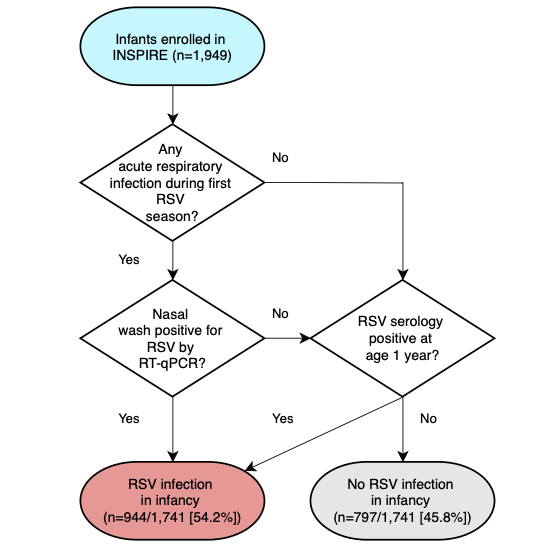
\includegraphics[scale=0.2]{f1}
	\caption{legend.}
	\label{fig:1}
\end{figure}

\begin{figure}[ht] \hspace*{0cm}
    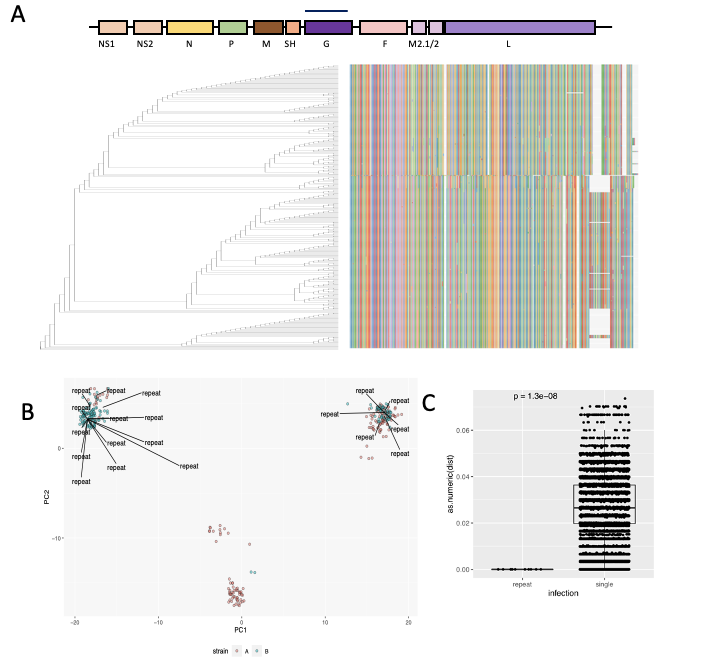
\includegraphics[scale=0.4]{f2}
	\caption{legend}
	\label{fig:2} \end{figure}

\begin{figure}[ht] \hspace*{0cm}
    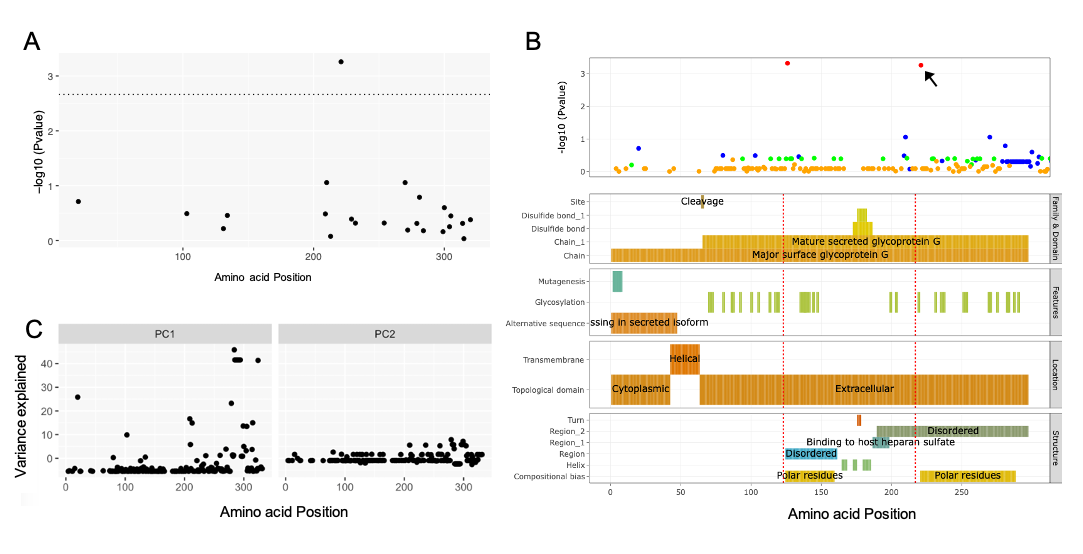
\includegraphics[scale=0.4]{f3}
	\caption{legend.}
	\label{fig:3} \end{figure}
	
	\begin{figure}[ht] \hspace*{0cm}
    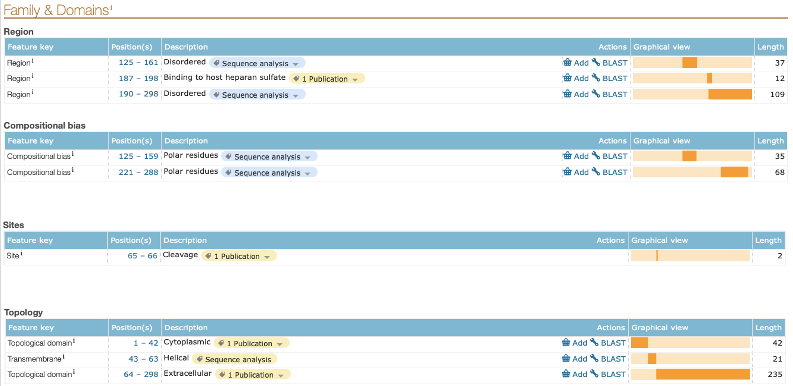
\includegraphics[scale=0.4]{f4}
	\caption{This is a place holder image. The figures are currently in adobe illustrator format: protein domain, structure - interaction, features.}
	\label{fig:4} \end{figure}
	
	\begin{figure}[ht] \hspace*{0cm}
    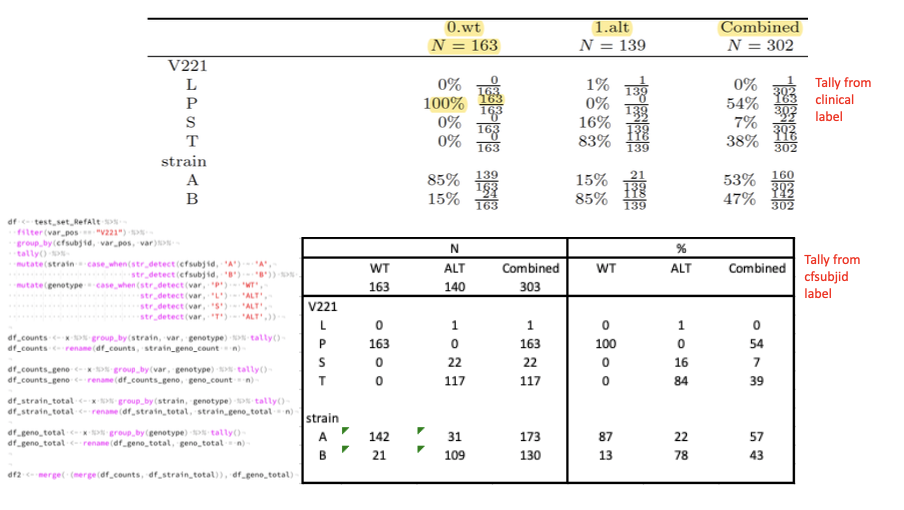
\includegraphics[scale=0.5]{fx}
	\caption{We do not need a table here - just a reminder of discussion with Tina.
	Is just the short result in text enough? IFN associated with strain A/B, and which cor with our variant, but unlikely due to our single variant 
	-- Yes - Tina agrees. .}
	\label{fig:5} \end{figure}
	
\end{document}
